\documentclass[11pt,a4paper]{article}
\usepackage[utf8]{inputenc}
\usepackage[spanish]{babel}	%Idioma
\usepackage{amsmath}
\usepackage{amsfonts}
\usepackage{amssymb}
\usepackage{graphicx} 	%Añadir imágenes
\usepackage{geometry}	%Ajustar márgenes
\usepackage[export]{adjustbox}[2011/08/13]
\usepackage{float}
\restylefloat{table}
\usepackage[hidelinks]{hyperref}
\usepackage{titling}
\graphicspath{{/home/nazaret/Escritorio/LaTEX}}
%\usepackage{minted}
\usepackage{multirow}
\usepackage{caption}
\usepackage{multicol}
\usepackage[shortlabels]{enumitem}
\usepackage{array}
\selectlanguage{spanish}

%Opciones de encabezado y pie de página:
\usepackage{fancyhdr}
\pagestyle{fancy}
\lhead{Nazaret Román Guerrero}
\rhead{Redes Multiservicio}
\lfoot{Grado en Ingeniería Informática}
\cfoot{}
\rfoot{\thepage}
\renewcommand{\headrulewidth}{0.4pt}
\renewcommand{\footrulewidth}{0.4pt}

%Opciones de fuente:
\usepackage[utf8]{inputenc}
\usepackage[default]{sourcesanspro}
\usepackage{sourcecodepro}
\usepackage[T1]{fontenc}

\setlength{\parindent}{15pt}
\setlength{\headheight}{15pt}
\setlength{\voffset}{10mm}

% Custom colors
\usepackage{color}
\definecolor{deepblue}{rgb}{0,0,0.5}
\definecolor{deepred}{rgb}{0.6,0,0}
\definecolor{deepgreen}{rgb}{0,0.5,0}

\usepackage{listings}

\begin{document}
\begin{titlepage}

\begin{minipage}{\textwidth}

\centering

\includegraphics[width=0.5\textwidth]{img/logo.png}\\

\textsc{\Large Redes Multiservicio\\[0.2cm]}
\textsc{GRADO EN INGENIERÍA INFORMÁTICA}\\[1cm]

{\Huge\bfseries Seminario 4: HTTP Video Streaming\\}
\noindent\rule[-1ex]{\textwidth}{3pt}\\[3.5ex]
{\large\bfseries Un caso de estudio: YouTube}
\end{minipage}

\vspace{1.5cm}
\begin{minipage}{\textwidth}
\centering

\textbf{Autora}\\ {Nazaret Román Guerrero}\\[2.5ex]

\includegraphics[width=0.3\textwidth]{img/etsiit.jpeg}\\[0.1cm]
\vspace{1cm}
\textsc{Escuela Técnica Superior de Ingenierías Informática y de Telecomunicación}\\
\vspace{1cm}
\textsc{Curso 2018-2019}
\end{minipage}
\end{titlepage}

\pagenumbering{gobble}
\pagenumbering{arabic}
\tableofcontents
\thispagestyle{empty}

\newpage

Para llevar a cabo el análisis he escogido una canción reciente, de hace 9 meses. El vídeo en YouTube está a 4k, así que es un buen ejemplo. El vídeo es \color{blue} \href{https://youtu.be/q0hyYWKXF0Q}{Dance Monkey}\color{black}. \\

Podemos ver unas primeras estadísiticas del vídeo, como el ID del vídeo, la velocidad de conexión, la descarga del vídeo o los códecs del vídeo y del audio con los correspondientes \textit{itags} entre paréntesis.

\begin{figure}[H]
	\centering
	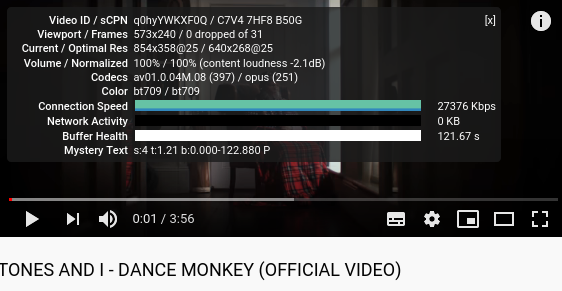
\includegraphics[scale=0.7]{img/nerds.png}
\end{figure}		

\section{Análisis sin estrangulamiento}

Vamos a analizar el vídeo sin estrangulamiento. Para ello, vamos a buscar el \textit{itag}, el \textit{mimetype} y el rango de bytes descargados.\\

Vamos a comenzar analizando el vídeo:

\begin{itemize}
	\item \textbf{\textit{itag}}: es un código numérico que indica el formato y resolución del vídeo. En nuestro caso es 397, lo que significa que es un vídeo mp4 con resolución 480p.
	
	\begin{figure}[H]
		\centering
		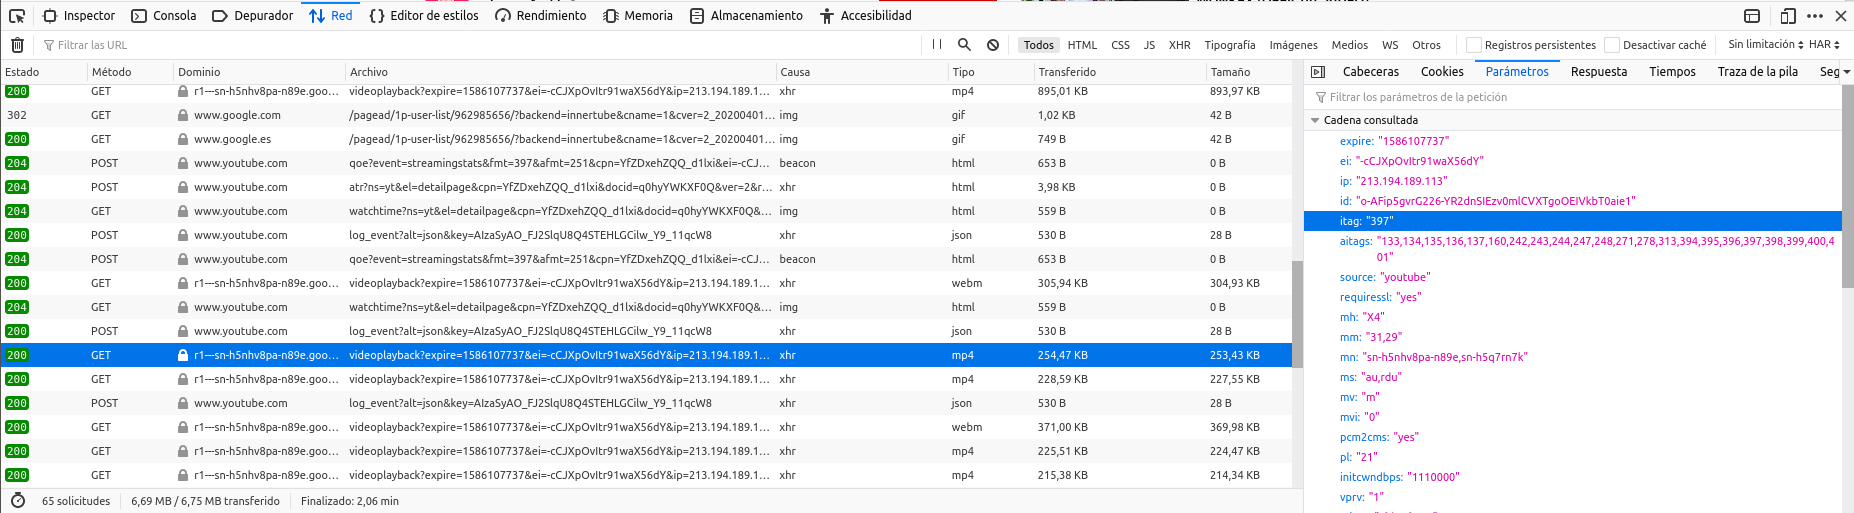
\includegraphics[scale=0.22]{img/itag.png}
	\end{figure}		
	
	\item \textbf{\textit{mime}}: indica el formato de vídeo. Esta información también se puede sacar con el \textit{itag} pero comprobando el \textit{mime} es una forma de asegurarnos. Nosotros tenemos un vídeo en formato mp4.
	
	\begin{figure}[H]
		\centering
		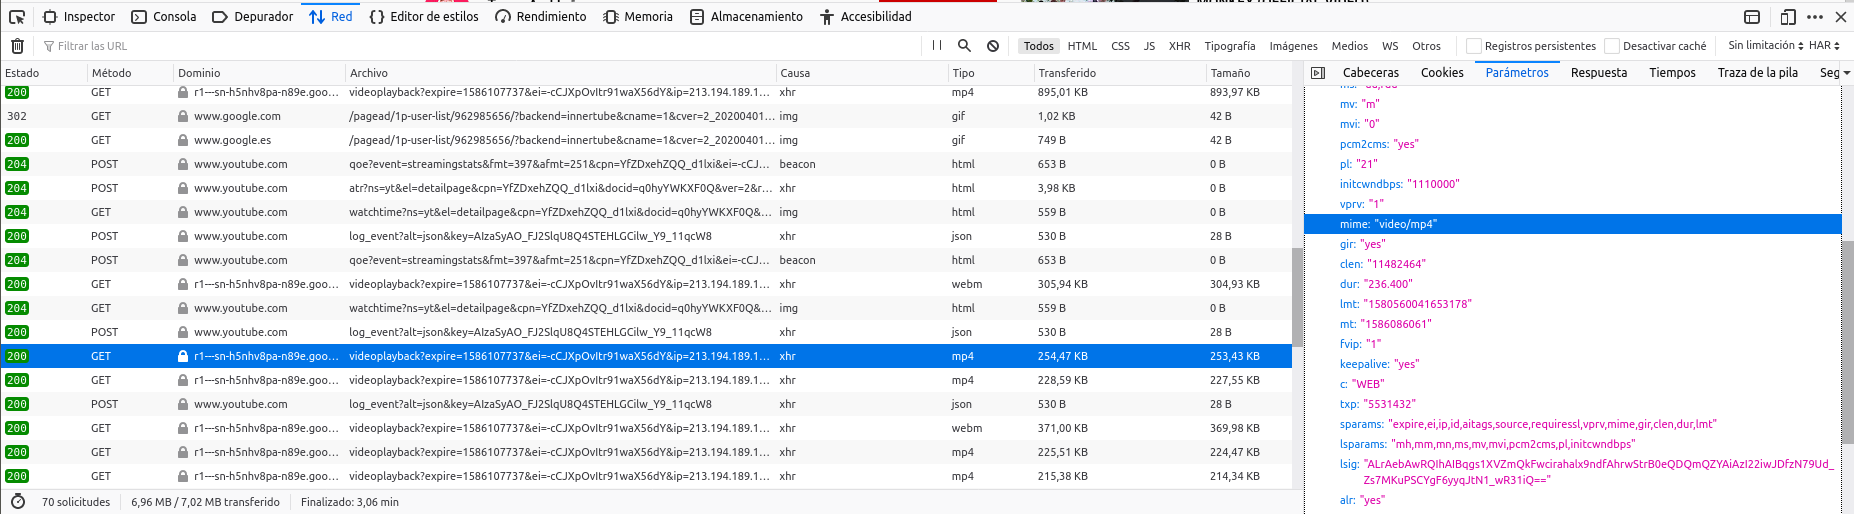
\includegraphics[scale=0.22]{img/mime.png}
	\end{figure}
	
	\item \textbf{\textit{range}}: indica el byte desde el que ha empezado la descarga hasta el byte final descargado. Como se puede ver en la imagen, se han descargado 259512 bytes, unos 253.4 KB.
	
	\begin{figure}[H]
		\centering
		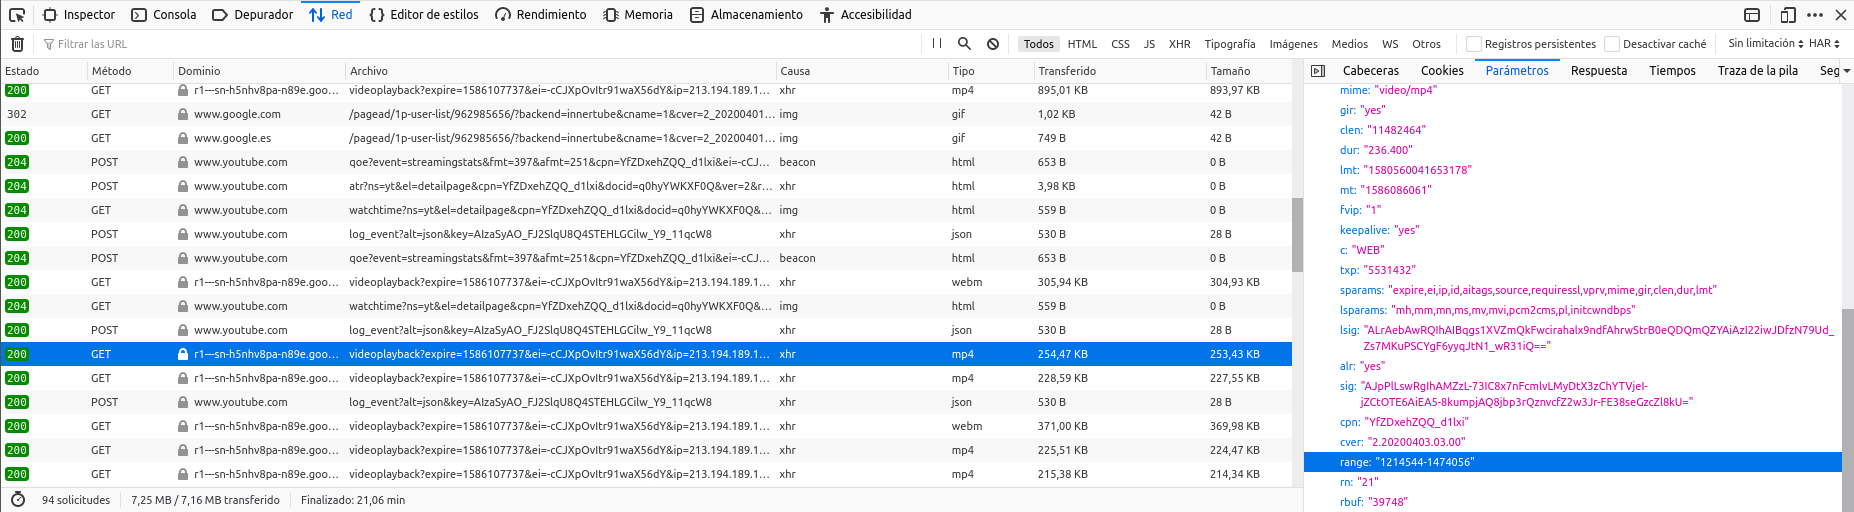
\includegraphics[scale=0.22]{img/range.png}
	\end{figure}		
	
\end{itemize}

Ahora que hemos analizado el vídeo, vamos a analizar el tráfico del audio. Vamos a utilizar los mismos parámetros de la petición HTTP que hemos usado con el vídeo:

\begin{itemize}
	\item \textbf{\textit{itag}}: indica el formato y resolución del audio. El nuestro es 251, es decir, es un audio en formato webm con un bitrate de 160k.
	
	\begin{figure}[H]
		\centering
		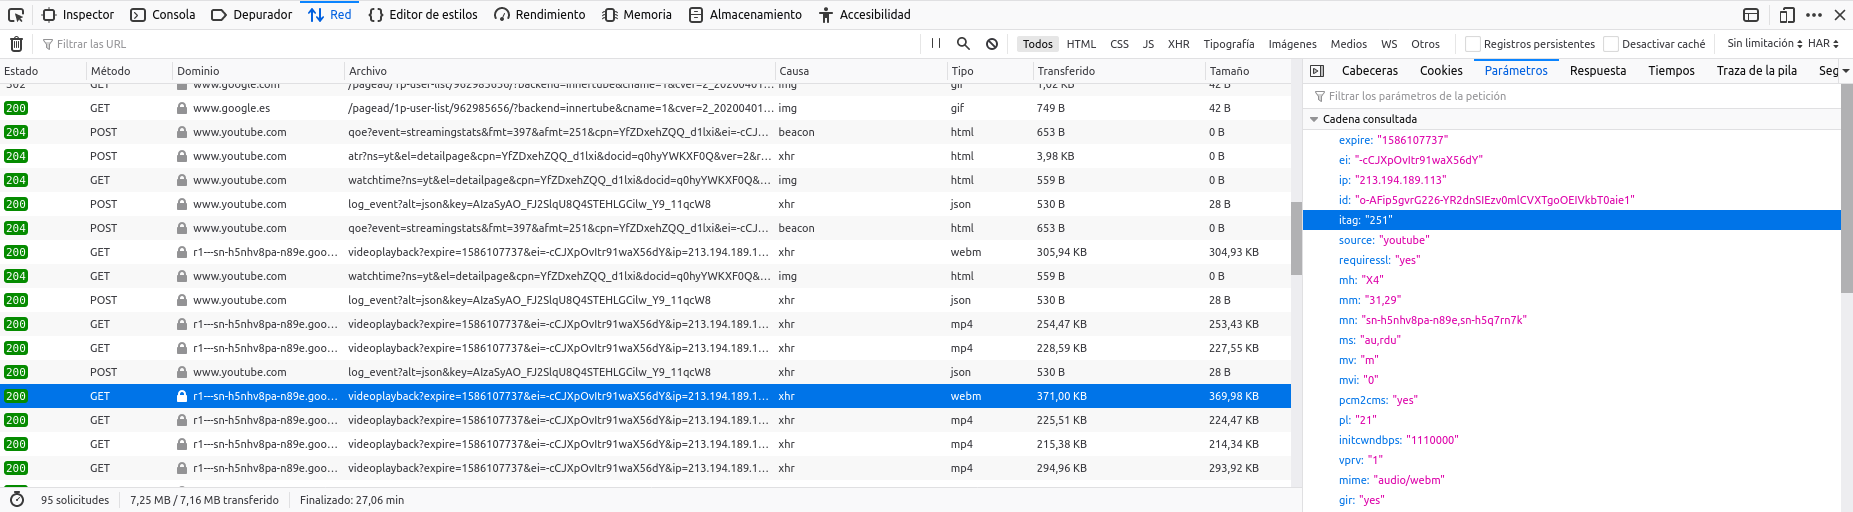
\includegraphics[scale=0.22]{img/audioitag.png}
	\end{figure}
	
	\item \textbf{\textit{mime}}: indica el formato del audio. En nuestro caso es webm.
	
	\begin{figure}[H]
		\centering
		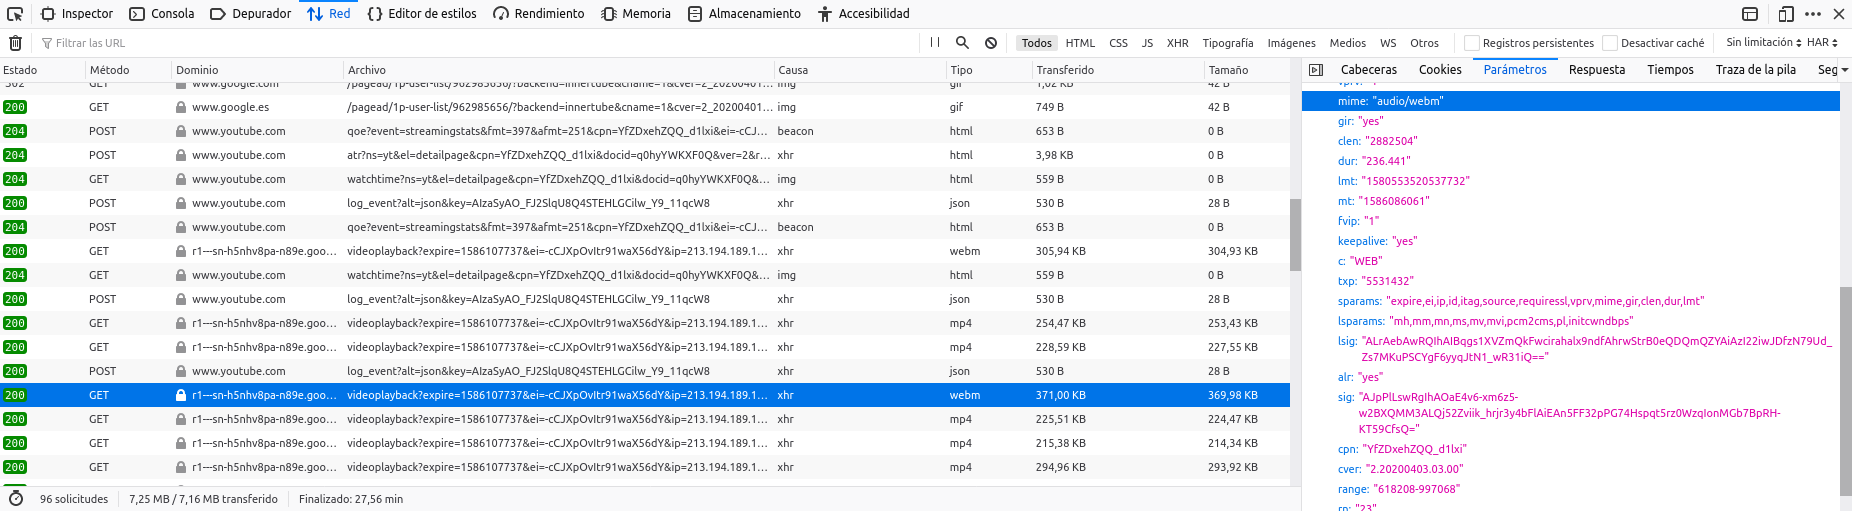
\includegraphics[scale=0.22]{img/audiomime.png}
	\end{figure}	
	
	\item \textbf{\textit{range}}: indica los bytes de audio descargados. En este fragmento se han descargado 378860 bytes, 370KB.
	
	\begin{figure}[H]
		\centering
		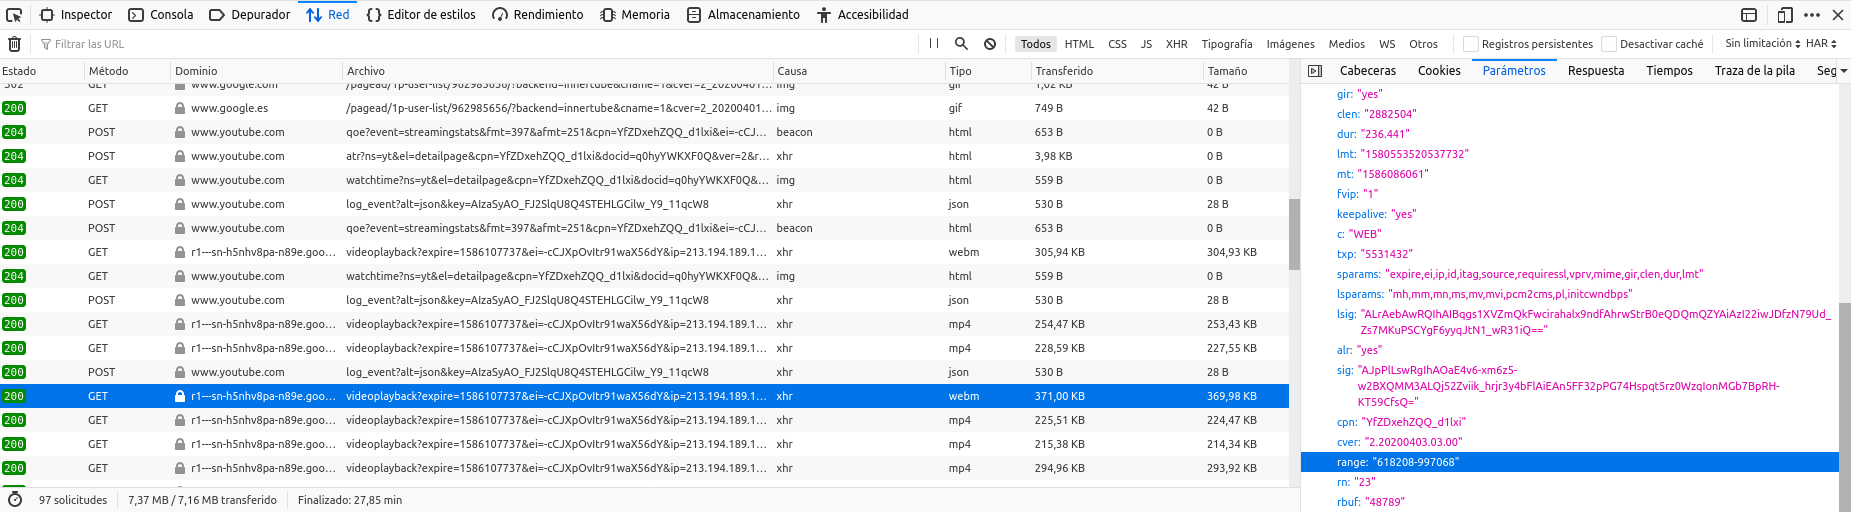
\includegraphics[scale=0.22]{img/rangeaudio.png}
	\end{figure}	
	
\end{itemize}

\section{Análisis con estrangulamiento}

Ahora vamos a utilizar la opción de estrangulamiento para poder comparar la descarga con y sin él. Yo he utiizado un estrangulamiento que supone una red 2G con una conexión normal, no una buena conexión (regular 2G).\\

Es importante decir antes que nada que al cambiar la conexión de red, el vídeo sufre muchas más pausas para poder cargar más bytes de vídeo y audio. Es decir, la calidad de experiencia se degrada notablemente.\\

Vamos a mostrar los mismos parámetros que antes pero con una red 2G:

\begin{itemize}
	\item \textbf{\textit{itag}}: el itag cambia en este caso para el vídeo pero no para el audio. El audio se mantiene con un \textit{itag} de 251, mientras que el vídeo se degrada a 395, que indica que es un vídeo mp4 pero con resolución 240p. Las siguientes imágenes muestran los \textit{itags} del vídeo y el audio respectivamente.
	
	\begin{figure}[H]
		\centering
		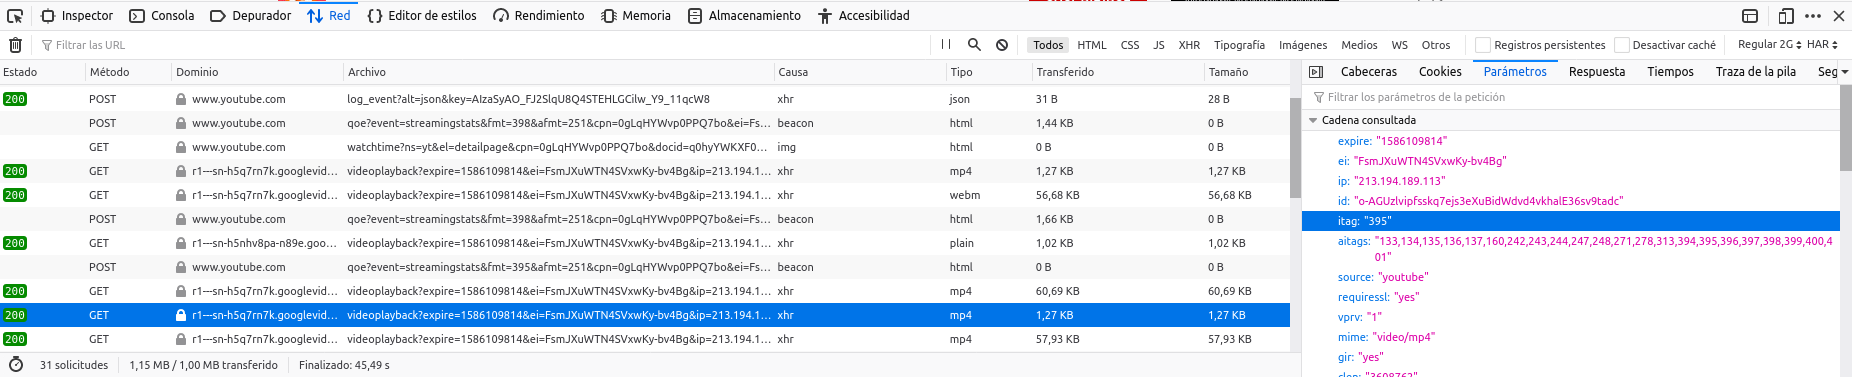
\includegraphics[scale=0.22]{img/itag2g.png}
	\end{figure}
	
	\begin{figure}[H]
		\centering
		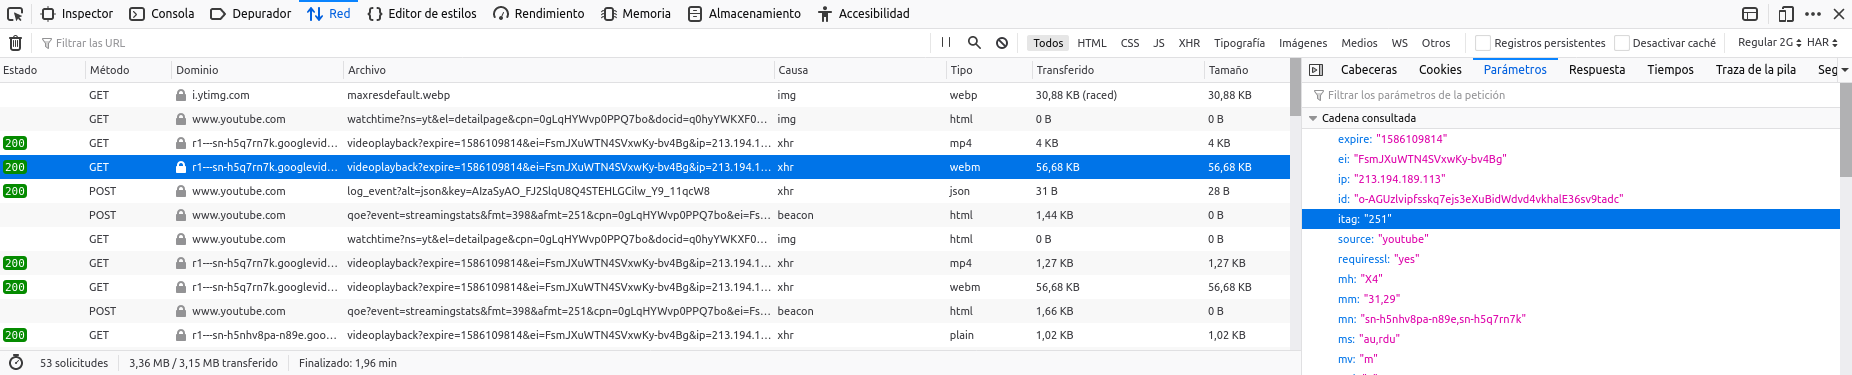
\includegraphics[scale=0.22]{img/itagaudio2g.png}
	\end{figure}
	
	\item \textbf{\textit{mime}}: ambos tipos se mantienen igual puesto que el formato no depende del estrangulamiento.
	
	\item \textbf{\textit{range}}: en este caso, tanto el vídeo como el audio experimentan sendas diferencias. El rango de descarga es mucho menor que en el caso sin estrangulamiento. El vídeo descarga solamente 1295 bytes, poco más de un KB, mientras que en el caso sin estrangulamiento se descargaban más de 250 KB. En el caso del audio se descargan 58040 bytes, unos 56 KB, que supone una diferencia de más de 300 KB respecto al caso sin estrangulamiento. En las imágenes siguientes se muestran los rangos del vídeo y el audio respectivamente.
	
	\begin{figure}[H]
		\centering
		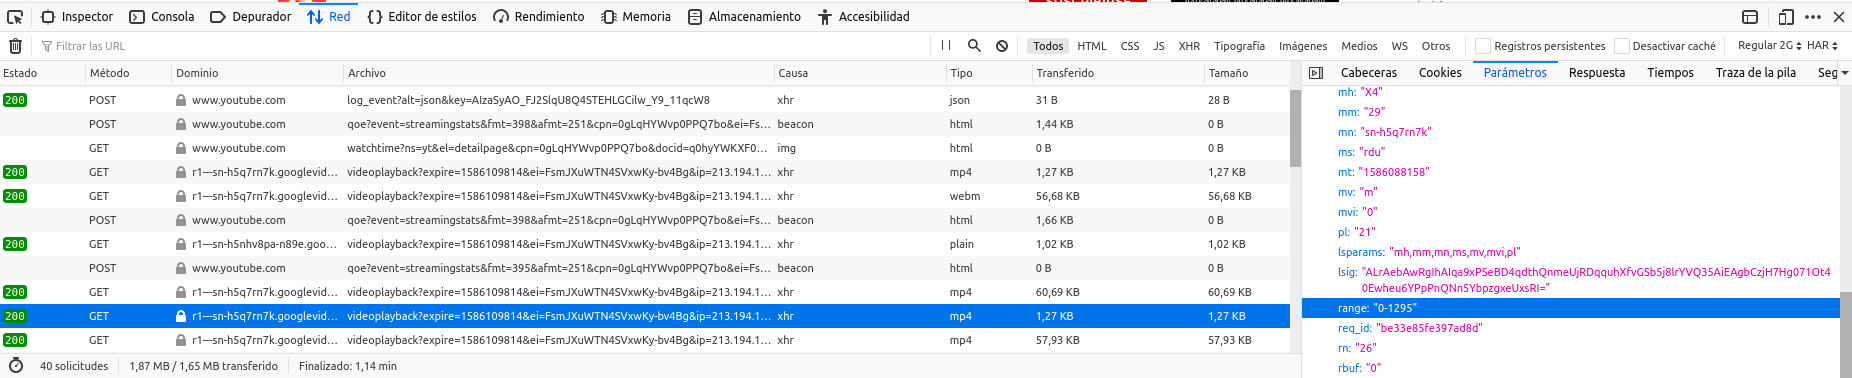
\includegraphics[scale=0.22]{img/range2g.png}
	\end{figure}
	
	\begin{figure}[H]
		\centering
		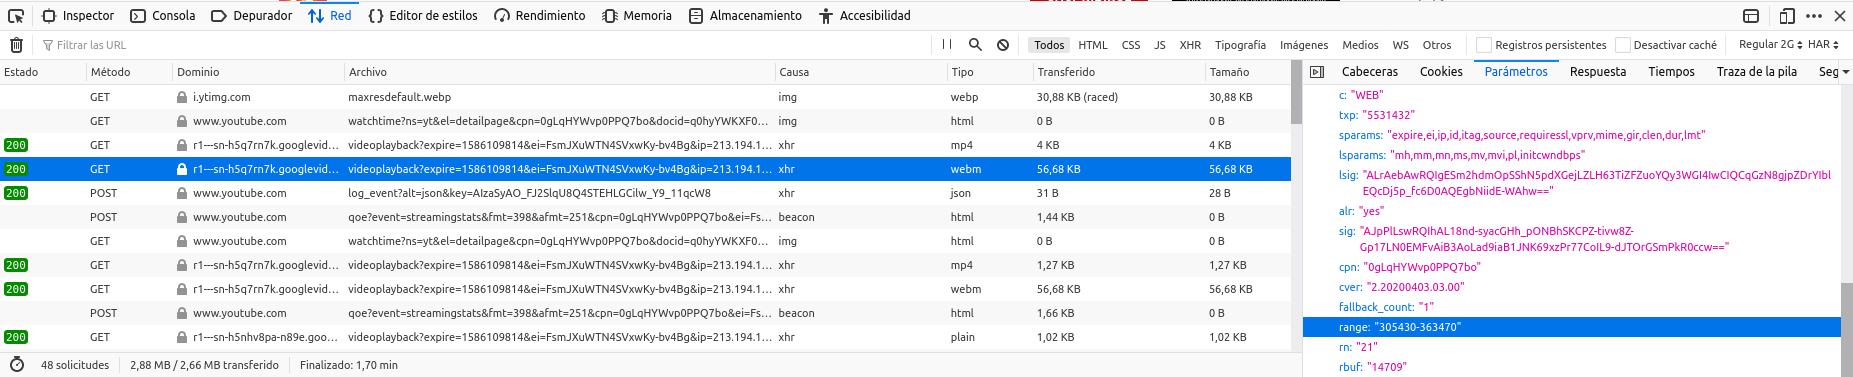
\includegraphics[scale=0.22]{img/rangeaudio2g.png}
	\end{figure}
		
\end{itemize}

Por tanto, hemos comprobado que la conexión influye en la calidad del vídeo y en la velocidad de descarga (por eso en el caso con estrangulamiento hay tantas pausas).

\end{document}